\section{双曲线}

本节要点:
\begin{itemize}
    \item 掌握双曲线的概念;
    \item 从代数角度掌握双曲线的几何性质。
\end{itemize}

%============================================================
\subsection{双曲线及其标准方程}

\begin{definition}[双曲线]
设二维平面中有两个定点$F_1,F_2$,若平面上的点和$F_1,F_2$的距离之差的绝对值都是$r>0$,则称这些点组成的集合为{\bf 双曲线},常用$H$表示,即:
\[
H:=\left\{ P \middle| \left| \left| \overrightarrow{F_1P} \right|-\left| \overrightarrow{F_2P} \right| \right|=r \right\}
\]
其中,$F_1,F_2$称为{\bf 焦点},$\left| \overrightarrow{F_1F_2} \right|$称为{\bf 焦距}。若令$F_1=\left( -c,0 \right) ,F_2=\left( c,0 \right) $,则双曲线可以表示为下列的{\bf 标准方程}:
\[
\frac{x^2}{a^2}-\frac{y^2}{b^2}=1
\]
其中$a,b,c$满足$a^2+b^2=c^2$。
\end{definition}

\begin{figure}[h]
\centering
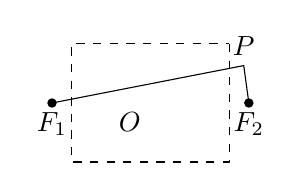
\begin{tikzpicture}[line join=round, scale=0.25]
\pgfmathparse{0.6/0.25}
\mydrawxy{-7}{7}{-5}{5}
\mydrawhyperbola{7}{4}{3}
\coordinate[label=below left:{$O$}]   (O)  at (0,0);
\coordinate[label=below:     {$F_1$}] (F1) at (-5,0);
\coordinate[label=below:     {$F_2$}] (F2) at (5,0);
\coordinate[label=above:     {$P$}]   (P)  at (4.74,1.90);
\fill (F1) circle (\pgfmathresult mm);
\fill (F2) circle (\pgfmathresult mm);
\draw (F1)--(P)--(F2);
\draw[dashed] (4,3)--(4,-3)--(-4,-3)--(-4,3)--(4,3);
\end{tikzpicture}
\end{figure}

\begin{tcolorbox}
详细阅读课本关于双曲线标准方程的推导过程,体会两次平方的意义。详细阅读例6,可以认为是双曲线的另外的定义。
\end{tcolorbox}

%============================================================
\subsection{双曲线的简单几何性质}

双曲线图形如下,我们称:
\begin{itemize}
    \item $O,A_1,A_2,B_1,B_2$:一个{\bf 中心}和四个{\bf 顶点};
    \item $A_1A_2=2a$:{\bf 实轴};
    \item $B_1B_2=2b$:{\bf 虚轴};
    \item $F_1F_2=2c$:{\bf 焦距};
    \item $e=\frac{c}{a}=\frac{1}{\cos \theta}\in \left( 1,+\infty \right) $:{\bf 离心率},$e$越大双曲线开口越大;
    \item $y=\pm \frac{b}{a}x$:{\bf 渐近线}。
\end{itemize}

\begin{figure}[h]
\centering
\begin{tikzpicture}[line join=round, scale=0.5]
\pgfmathparse{0.6/0.5}
\mydrawxy{-7}{7}{-5}{5}
\mydrawhyperbola{7}{4}{3}
\coordinate[label=below left: {$O$}]   (O)  at (0,0);
\coordinate[label=below:      {$F_1$}] (F1) at (-5,0);
\coordinate[label=below:      {$F_2$}] (F2) at (5,0);
\coordinate[label=below right:{$A_1$}] (A1) at (-4,0);
\coordinate[label=below left: {$A_2$}] (A2) at (4,0);
\coordinate[label=above left: {$B_1$}] (B1) at (0,3);
\coordinate[label=below left: {$B_2$}] (B2) at (0,-3);
\fill (F1) circle (\pgfmathresult mm);
\fill (F2) circle (\pgfmathresult mm);
\draw[dashed] ($(A2)+(B1)$)--($(A2)+(B2)$)--($(A1)+(B2)$)--($(A1)+(B1)$)--($(A2)+(B1)$);
\draw[dashed] ($(O)!1.7!($(A1)+(B2)$)$)--($(O)!1.7!($(A2)+(B1)$)$) ($(O)!1.7!($(A1)+(B1)$)$)--($(O)!1.7!($(A2)+(B2)$)$);
\coordinate[label=above:{$a$}] (a) at ($(0,3)!0.5!(4,3)+(0,0.5)$);
\draw[decorate,decoration={calligraphic brace,raise=0cm,aspect=0.5,amplitude=0.2cm},thick] (0,3)--(4,3);
\coordinate[label=right:{$b$}] (b) at ($(4,3)!0.5!(4,0)+(0.5,0)$);
\draw[decorate,decoration={calligraphic brace,raise=0cm,aspect=0.5,amplitude=0.2cm},thick] (4,3)--(4,0);
\coordinate (t) at (4,3);
\pic["$\theta $",draw,angle radius=0.5cm,angle eccentricity=1.5] {angle=F2--O--t};
\end{tikzpicture}
\end{figure}

%============================================================
\subsection{拓展讨论:坐标系变换}

同椭圆,略。

%============================================================
\subsection{拓展讨论:斜率之积}

设双曲线$H$及双曲线上一点$P$,则$PA_1,PA_2$的斜率之积有:
\begin{align*}
&\because \frac{x^2}{a^2}-\frac{y^2}{b^2}=1 \\
&\therefore k_{PA_1}k_{PA_2}=\frac{y_P}{x_P+a}\cdot \frac{y_P}{x_P-a}=\frac{b^2\left( \frac{{x_P}^2}{a^2}-1 \right)}{{x_P}^2-a^2}=\frac{b^2}{a^2}=\tan ^2\theta
\end{align*}

\begin{figure}[h]
\centering
\begin{tikzpicture}[line join=round, scale=0.25]
\pgfmathparse{0.6/0.25}
\mydrawxy{-7}{7}{-5}{5}
\mydrawhyperbola{7}{4}{3}
\coordinate[label=below left: {$O$}]   (O)  at (0,0);
\coordinate[label=below:      {$F_1$}] (F1) at (-5,0);
\coordinate[label=below:      {$F_2$}] (F2) at (5,0);
\coordinate[label=below right:{$A_1$}] (A1) at (-4,0);
\coordinate[label=below left: {$A_2$}] (A2) at (4,0);
\coordinate[label=above:      {$P$}]   (P)  at (6.20,3.56);
\fill (F1) circle (\pgfmathresult mm);
\fill (F2) circle (\pgfmathresult mm);
\draw (A1)--(P)--(A2);
\draw[dashed] ($(O)!1.7!(-4,-3)$)--($(O)!1.7!(4,3)$) ($(O)!1.7!(-4,3)$)--($(O)!1.7!(4,-3)$);
\coordinate (t) at (4,3);
\pic["$\theta $",draw,angle radius=0.5cm,angle eccentricity=1.5] {angle=F2--O--t};
\end{tikzpicture}
\end{figure}

%============================================================
\subsection{拓展讨论:两个焦点}

从任意一个焦点出发的光线都可以视作从另一个焦点发出,证明这点需要微积分的知识,略。

\begin{figure}[ht]
\centering
\begin{tikzpicture}[line join=round, scale=0.25]
\pgfmathparse{0.6/0.25}
\mydrawxy{-7}{7}{-5}{5}
\mydrawhyperbola{7}{4}{3}
\coordinate[label=below left:{$O$}]   (O)  at (0,0);
\coordinate[label=below:     {$F_1$}] (F1) at (-5,0);
\coordinate[label=below:     {$F_2$}] (F2) at (5,0);
\coordinate                           (P1) at (5.23,2.53);
\coordinate                           (P2) at (4.42,1.41);
\coordinate                           (P3) at (4.43,-1.43);
\fill (F1) circle (\pgfmathresult mm);
\fill (F2) circle (\pgfmathresult mm);
\draw (F2)--(P1) (F2)--(P2) (F2)--(P3);
\draw[dashed] (F1)--(P1) (F1)--(P2) (F1)--(P3);
\draw (P1)--($(P1)!-0.8!(F1)$) (P2)--($(P2)!-1.0!(F1)$) (P3)--($(P3)!-1.0!(F1)$);
\end{tikzpicture}
\end{figure}

%============================================================
\subsection{拓展讨论:动点距离直线}

\begin{tcolorbox}
对课本例5深入讨论。
\end{tcolorbox}

我们考察,对于任意一个椭圆$E$,是否必有垂直坐标轴的直线$x=x_0$,且椭圆上的点$P$距离焦点和直线的比是定值$k$。

\begin{figure}[h]
\centering
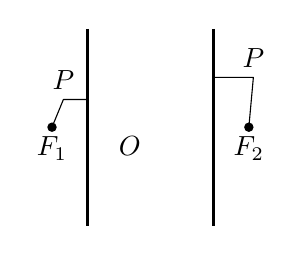
\begin{tikzpicture}[line join=round, scale=0.25]
\pgfmathparse{0.6/0.25}
\mydrawxy{-7}{7}{-5}{5}
\mydrawhyperbola{7}{4}{3}
\coordinate[label=below left:{$O$}]   (O)  at (0,0);
\coordinate[label=below:     {$F_1$}] (F1) at (-5,0);
\coordinate[label=below:     {$F_2$}] (F2) at (5,0);
\coordinate[label=above:     {$P$}]   (P1) at (-4.42,1.41);
\coordinate[label=above:     {$P$}]   (P2) at (5.23,2.53);
\fill (F1) circle (\pgfmathresult mm);
\fill (F2) circle (\pgfmathresult mm);
\draw[thick] (-3.2,5)--(-3.2,-5) (3.2,5)--(3.2,-5);
\draw (-3.2,1.41)--(P1)--(F1);
\draw (3.2,2.53)--(P2)--(F2);
\end{tikzpicture}
\end{figure}

距离焦点和直线的比:
\begin{align*}
&\frac{x^2}{a^2}-\frac{y^2}{b^2}=1 \\
&k=\frac{\sqrt{\left( x\pm c \right) ^2+y^2}}{\left| x-x_0 \right|}\Rightarrow k^2\left( x-x_0 \right) ^2=\left( x\pm c \right) ^2+y^2
\end{align*}
化简后得:
\[
\left( 1-k^2+\frac{b^2}{a^2} \right) x^2+2\left( k^2x_0\pm c \right) x+\left( a^2-k^2{x_0}^2 \right) =0
\]
若要对所有$x$都成立,必须:
\[
\begin{cases}
	1-k^2+\frac{b^2}{a^2}=0\\
	k^2x_0\pm c=0\\
	a^2-k^2{x_0}^2=0\\
\end{cases}\Rightarrow \quad \begin{cases}
	k=\frac{c}{a}\in \left( 1,+\infty \right) \\
	x_0=\mp \frac{a^2}{c}\\
\end{cases}
\]
不难发现特点:
\begin{itemize}
    \item 对于左焦点有左边的直线$x=-\frac{a^2}{c}$,对于右焦点有右边的直线$x=\frac{a^2}{c}$,且两条直线一定在双曲线内侧;
    \item 动点距离直线更近。
\end{itemize}

%============================================================
\subsection{拓展讨论:双曲线的一般方程}

我们来推导一下双曲线方程的一般形式。中心点平移的讨论见椭圆,我们直接从旋转开始。双曲线的采用极坐标的形式,双曲线绕中心点沿顺时针转$\alpha $后的方程如下:
\[
\frac{\left[ r\cos \left( \theta -\alpha \right) \right] ^2}{a^2}-\frac{\left[ r\sin \left( \theta -\alpha \right) \right] ^2}{b^2}=1 \qquad \alpha \in \left[ 0,\pi \right)
\]
注意我们这里是顺时针转动图形,相当于逆时针转动坐标系,所以是$-\alpha $而不是$+\alpha $,展开后:
\begin{align*}
&\left( b^2\cos ^2\alpha -a^2\sin ^2\alpha \right) x^2+\left( b^2\sin ^2\alpha -a^2\cos ^2\alpha \right) y^2+c^2\sin 2\alpha xy=a^2b^2 \\
&Ax^2+By^2+Cxy+F=0 \\
&\begin{cases}
	A=b^2\cos ^2\alpha -a^2\sin ^2\alpha =\frac{c^2}{2}\left( 1+\cos 2\alpha \right) -a^2\\
	B=b^2\sin ^2\alpha -a^2\cos ^2\alpha =\frac{c^2}{2}\left( 1-\cos 2\alpha \right) -a^2\\
	C=c^2\sin 2\alpha\\
	F=-a^2b^2\\
\end{cases}
\end{align*}
不难发现:
\begin{itemize}
    \item $F<0$,若$F>0$则曲线不存在,若$F=0$则有可能是一点有可能是直线,这点同椭圆;
    \item $A+B=b^2-a^2,A-B=c^2\cos 2\alpha $,当$A=B$时$\alpha =\pi /4$或$3\pi /4$。
\end{itemize}
特别地,当$\alpha =\pi /4$时,方程为在圆的基础上加一个$xy$项,如下:
\[
\frac{b^2-a^2}{2}x^2+\frac{b^2-a^2}{2}y^2+c^2xy=a^2b^2
\]
当$\alpha =\pi /2$时,表现为实轴虚轴互换,如下:
\[
-a^2x^2+b^2y^2=a^2b^2
\]

%============================================================
\subsection{拓展讨论:\texorpdfstring{$y=\frac{1}{x}$}{y=1/x}和\texorpdfstring{$y=x+\frac{1}{x}$}{y=x+1/x}}

继续上面的讨论,若有$a=b=\sqrt{2}$,则双曲线为:
\[
\frac{x^2}{2}-\frac{y^2}{2}=1
\]
显然$y=\pm x$是它的两条渐近线。当我们沿顺时针旋转$\pi /4$后:
\begin{align*}
&\frac{b^2-a^2}{2}x^2+\frac{b^2-a^2}{2}y^2+c^2xy=a^2b^2 \\
&\because a=b=\sqrt{2},c=2 \\
&\therefore xy=1
\end{align*}
这也是为什么之前碰到的$y=\frac{1}{x}$也称为双曲线的原因。

\begin{figure}[h]
\centering
\begin{tikzpicture}[line join=round, scale=0.25]
\pgfmathparse{0.6/0.25}
\mydrawxy{-7}{7}{-5}{5}
\mydrawhyperbola{5}{1.414}{1.414}
\draw[thick,domain=0.2:5,samples=200]   plot (\x,{1/\x});
\draw[thick,domain=-5:-0.2,samples=200] plot (\x,{1/\x});
\end{tikzpicture}
\end{figure}

对于$y=x+\frac{1}{x}$,两边同乘以$x$可得:
\[
x^2-xy+1=0
\]
其实就是压缩了开口,再沿顺时针转$3\pi /8$,具体分析略,可借助GeoGebra研究其变化。

%============================================================
\subsection{习题}

\begin{example}[综合运用11,难度:$\star $]
$M$是一个动点,$MA$与直线$y=x$垂直,垂足$A$位于第一象限,$MB$与直线$y=-x$垂直,垂足$B$位于第四象限。若四边形$OAMB$($O$为原点)的面积为3,求动点$M$的轨迹方程。
\end{example}

解:

本题一步步解不难,略。实际为图象$xy=3$绕原点按顺时针转$\pi /4$,自然是双曲线。

我们要考察的是若这两条线为任意的$y_1=k_1x,y_2=k_2x$,以动点和原点加上这两条直线组成的平行四边形$OAMB$的面积为定值$S$,动点$M$的轨迹方程是否为双曲线。根据上面的讨论,其实是双曲线,$y_1=k_1x,y_2=k_2x$是两条渐近线。

\begin{tcolorbox}
本题本身没有难度,但之后我们的思考很有意思。
\end{tcolorbox}

~

\begin{example}[拓广探索13,难度:$\star $]
已知双曲线$x^2-\frac{y^2}{2}=1$,过点$P\left( 1,1 \right) $的直线$l$与双曲线相交于$A,B$两点,$P$能否是线段$AB$的中点?为什么?
\end{example}

解:

易得$P$在双曲线中间,于是可设直线:
\[
y-1=k\left( x-1 \right)
\]
带入双曲线方程,求得交点坐标:
\[
x=\frac{k\left( 1-k \right) \pm \sqrt{k^2\left( 1-k \right) ^2+\left( 2-k^2 \right) \cdot \left[ \left( 1-k \right) ^2+2 \right]}}{\left( 2-k^2 \right)}
\]
若有焦点,则通过中心点求得$k$:
\[
x=\frac{k\left( 1-k \right)}{2-k^2}=1\Rightarrow k=2
\]
验证此时:
\[
\varDelta =4+\left( -2 \right) \cdot 3<0
\]
实际无交点,所以没有这样的直线。

\begin{tcolorbox}
本题没有难度。
\end{tcolorbox}

~

\begin{example}[拓广探索14,难度:$\star \star $]
一直双曲线$\frac{x^2}{4}-\frac{y^2}{16}=1$与直线$l:y=kx+m,k\ne \pm 2$有唯一的公共点$M$,过点$M$且与$l$垂直的直线分别交{\it x}轴、{\it y}轴于$A\left( x,0 \right) ,B\left( 0,y \right) $两点。当点$M$运动时,求点$P\left( x,y \right) $的轨迹方程,并说明轨迹是什么曲线。如果推广到一般双曲线,能得到什么相应的结论?
\end{example}

解:

将直线带入双曲线得到:
\[
\left( 4-k^2 \right) x^2-2kmx-\left( m^2+16 \right) =0
\]
根据题意要求:
\begin{align*}
&\varDelta =16\left( m^2-4k^2+16 \right) =0\Rightarrow m^2=4\left( k^2-4 \right) \\
&x_{1,2}=\frac{km\pm 2\sqrt{m^2-4k^2+16}}{4-k^2}
\end{align*}
得到$M$坐标:
\[
M=\left( x_M,y_M \right) =\left( -\frac{4k}{m},-\frac{16}{m} \right)
\]
于是过$M$垂直于$l$的直线:
\[
y+\frac{16}{m}=-\frac{1}{k}\left( x+\frac{4k}{m} \right)
\]
$P$坐标:
\[
P=\left( x_{y=0},y_{x=0} \right) =\left( -\frac{20k}{m},-\frac{20}{m} \right)
\]
是一个参数方程,结合$\varDelta =0$可化简为:
\[
\frac{x^2}{100}-\frac{y^2}{25}=1
\]
题中的一个交点显然$l$是双曲线的切线,又由于$l$是通过斜距式给出,所以$k\in \left( -\infty ,-2 \right) \cup \left( 2,+\infty \right) $,所以$P$的轨迹是双曲线但是不包括顶点。

对于一般的双曲线方程,有:
\begin{align*}
&H:\frac{x^2}{a^2}-\frac{y^2}{b^2}=1 \\
&H\cap l:\left( b^2-a^2k^2 \right) x^2-2a^2kmx-\left( a^2m^2+a^2b^2 \right) =0 \\
&x_{1,2}=\frac{a^2km\pm ab\sqrt{b^2+m^2-a^2k^2}}{b^2-a^2k^2}\text{且}-m^2=b^2-a^2k^2 \\
&M=\left( x_M,y_M \right) =\left( -\frac{a^2k}{m},-\frac{b^2}{m} \right) \\
&l_{\bot}:y+\frac{b^2}{m}=-\frac{1}{k}\left( x+\frac{a^2k}{m} \right) \\
&P=\left( -\frac{\left( a^2+b^2 \right) k}{m},-\frac{a^2+b^2}{m} \right)
\end{align*}

\begin{tcolorbox}
本题思路明显,但是计算量大。
\end{tcolorbox}




